\RequirePackage{silence}
\WarningFilter{memoir}{\settocpreprocessor}
\WarningFilter{microtype}{Unable to apply patch `footnote'}
\WarningFilter{listings}{First Aid}

\documentclass[12pt, openany, oneside, a4paper, brazilian]{abntex2}
% =========================================================
% PACOTES
% =========================================================

\usepackage[T1]{fontenc}
\usepackage[utf8]{inputenc}
\usepackage{lmodern}

\usepackage{indentfirst}
\usepackage[nopatch=footnote]{microtype}

\usepackage{graphicx}
\usepackage{pdfpages}
\usepackage{xcolor}
\usepackage{float}
\usepackage{booktabs}
\usepackage{multirow}
\usepackage{array}
\usepackage{amsmath}
\usepackage{tikz}
\usepackage{textcomp}
\usepackage{hyperref}

\usepackage[brazilian,hyperpageref]{backref}
\usepackage[alf]{abntex2cite}

\graphicspath{{imagens/}}

% =========================================================
% LISTINGS JAVA/C++
% =========================================================

\usepackage{listings}

\definecolor{javakeyword}{RGB}{0,0,180}
\definecolor{javacomment}{RGB}{63,127,95}
\definecolor{javastring}{RGB}{163,21,21}
\definecolor{javabg}{RGB}{248,248,248}

\lstdefinestyle{arduinoStyle}{
    language=C++,
    backgroundcolor=\color{javabg},
    basicstyle=\ttfamily\small,
    keywordstyle=\color{javakeyword}\bfseries,
    commentstyle=\color{javacomment}\itshape,
    stringstyle=\color{javastring},
    numberstyle=\tiny\color{gray},
    numbers=left,
    stepnumber=1,
    numbersep=8pt,
    showspaces=false,
    showstringspaces=false,
    showtabs=false,
    frame=single,
    rulecolor=\color{gray},
    tabsize=4,
    breaklines=true,
    breakatwhitespace=true,
    captionpos=b
}

\lstset{style=arduinoStyle}

% =========================================================
% INFORMAÇÕES DO TRABALHO
% =========================================================

\instituicao{
Centro Universitário Senac \par
Análise e Desenvolvimento de Sistemas \par
Disciplina: Conceitos de computação
}

\autor{Altino Ávila \\ Guilherme Diniz \\ 
Samuel \\ Jessiê}

\titulo{
Lixeira Automática utilizando Arduino Uno
}

\preambulo{
Tecnologia Frugal
}

\orientador{
Fábio Brussolo
}

\tipotrabalho{
Projeto
}

\local{
São Paulo
}

\data{
2026
}

% =========================================================
% DOCUMENTO
% =========================================================

\begin{document}

\selectlanguage{brazilian}
\frenchspacing

\imprimircapa
\imprimirfolhaderosto

\pdfbookmark[0]{\contentsname}{toc}
\tableofcontents*
\cleardoublepage

% =========================================================
% INTRODUÇÃO
% =========================================================

\chapter{Introdução}

\section{Contextualização do Projeto}

Link do projeto que utilizamos como base:\\ \url{https://www.youtube.com/watch?v=h7AmHDmgpJY}
\\
O presente projeto propõe o desenvolvimento de uma lixeira automática
baseada em Arduino Uno, utilizando sensor ultrassônico HC-SR04 para
detecção de proximidade e servo motor SG90 para acionamento automático
da tampa.

Este protótipo representa a 

\textbf{Fase 1} (automação local). Toda a estrutura de sensores e a lógica de programação foram desenvolvidas com o intuito de preparar o terreno para a \textbf{Fase 2}. Essa futura fase incluirá um módulo com conectividade Wi-Fi (como o ESP32) para enviar dados para a internet, avisando no celular, por exemplo, quando a lixeira estiver cheia.

\section{O Conceito de Tecnologia Frugal}


O nosso projeto adota o preceito da \textbf{Tecnologia Frugal}. Em termos simples, isso significa \textit{fazer mais com menos}. É uma abordagem voltada para criar soluções eficientes, acessíveis e de baixo custo, sem perder a funcionalidade.

Em vez de utilizarmos estruturas caras de metal impresso em 3D ou plásticos sob medida, aplicamos o conceito frugal utilizando papelão (material reciclável e de fácil acesso) para a montagem física da lixeira, combinado com eletrônica de entrada. O objetivo é provar que é possível criar automação inteligente gastando muito pouco.

\section{Objetivos do Projeto}

Os objetivos deste projeto são:

\begin{enumerate}
    \item Desenvolver uma lixeira automática funcional utilizando Arduino Uno;
    \item Implementar abertura automática sem contato físico;
    \item Utilizar sensores ultrassônicos para detecção de presença;
    \item Controlar a tampa utilizando servo motor SG90;
    \item Implementar fechamento automático temporizado;
    \item Criar uma base para futuras integrações IoT;
\end{enumerate}


% =========================================================
% FUNDAMENTAÇÃO TEÓRICA
% =========================================================

\chapter{Fundamentação Teórica}

\section{Arduino Uno}

O Arduino Uno é uma plataforma de prototipagem eletrônica baseada no
microcontrolador ATmega328P. A placa possui 14 portas digitais,
6 entradas analógicas e clock de 16 MHz. Funciona como o \textit{cérebro} do nosso projeto, coordenando os sensores e os motores.

\section{Sensor Ultrassônico HC-SR04}

O HC-SR04 é um sensor capaz de medir distâncias utilizando ondas ultrassônicas de 40 kHz. 

\textbf{Como explicar de forma simples:} Ele funciona exatamente como a ecolocalização de um morcego ou o sonar de um submarino. O sensor \textit{grita} um som muito agudo (que não conseguimos ouvir) e conta quanto tempo o eco demora para bater na mão de uma pessoa e voltar. Sabendo o tempo da viagem do som, o Arduino calcula a distância exata.

O módulo possui quatro pinos:
\begin{itemize}
    \item VCC (Energia);
    \item GND (Terra);
    \item Trigger (O \textit{alto-falante} que envia o pulso sonoro);
    \item Echo (O \textit{microfone} que escuta o retorno).
\end{itemize}

\section{Servo Motor SG90}

O SG90 é um micro servo motor utilizado para controle angular. Seu funcionamento ocorre através de sinais enviados pelo Arduino.

\textbf{Como explicar de forma simples:} Diferente do motor de um carrinho de controle remoto que fica girando sem parar, o servo motor funciona mais como a articulação de um \textit{braço robótico}. Ele sabe exatamente em qual ângulo está posicionado e consegue mover a tampa da lixeira controladamente do ponto A (fechada) ao ponto B (aberta), e parar lá.


% =========================================================
% ESPECIFICAÇÕES DO SISTEMA
% =========================================================

\chapter{Especificações do Sistema}

\section{Requisitos Funcionais}

\begin{enumerate}
    \item Detectar presença em até 20 cm;
    \item Abrir automaticamente a tampa;
    \item Fechar automaticamente após 5 segundos;
    \item Registrar eventos via Serial Monitor.
\end{enumerate}

\section{Requisitos Não-Funcionais}

\begin{itemize}
    \item Baixo consumo energético;
    \item Tempo de resposta inferior a 1 segundo;
    \item Fácil manutenção;
    \item Baixo custo de implementação;
    \item Funcionamento estável em ambientes internos.
\end{itemize}

\section{Lista de Componentes}

\begin{table}[H]
\centering
\caption{Lista de Componentes}
\begin{tabular}{lcc}
\toprule
Componente & Quantidade & Custo Médio (R\$) \\
\midrule
Arduino Uno & 1 & 35,00 \\
HC-SR04 & 1 & 19,00 \\
Servo SG90 & 1 & 20,00 \\
Kit Jumpers & 20 & 28,00 \\
\bottomrule
\end{tabular}
\end{table}

\section{Diagrama de Conexões Eletrônicas}

O sistema é composto por um sensor ultrassônico conectado ao
Arduino Uno, responsáveis pela detecção de presença.
O servo motor recebe os dados da distância medida e abre/fecha
a tampa.

\begin{figure}[H]
    \centering
    \caption{Diagrama de conexões elétricas e montagem do sistema}
    \label{fig:diagrama_conexoes}
    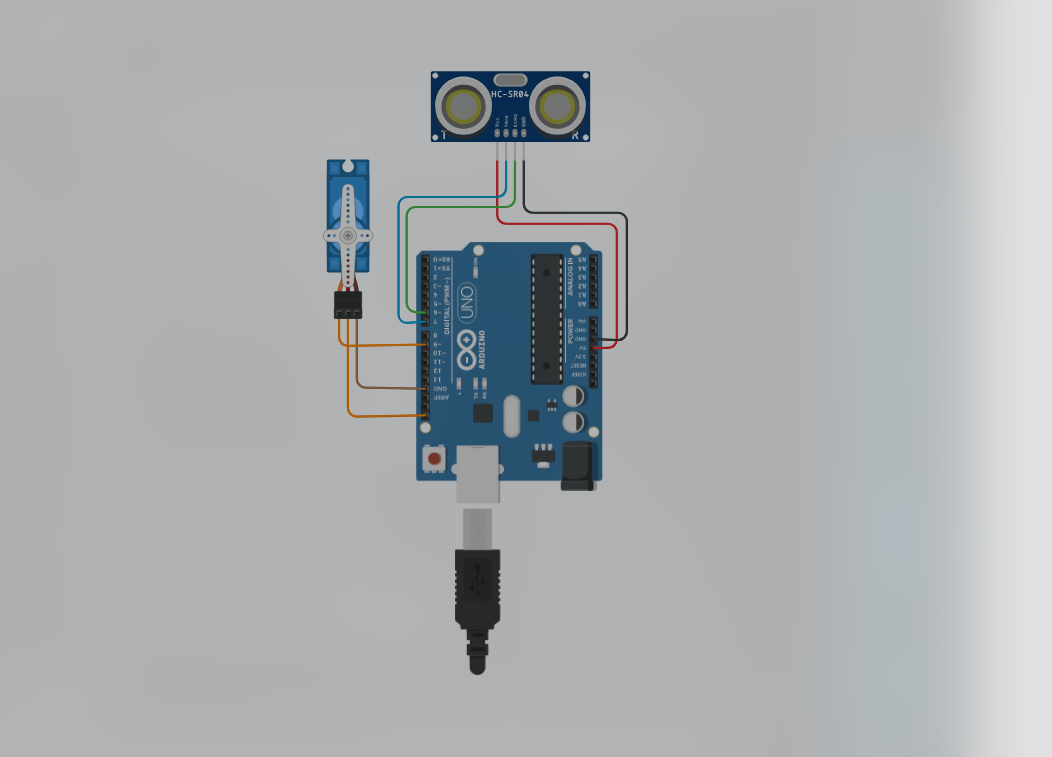
\includegraphics[width=0.85\textwidth]{uno} 
    \fonte{Adaptado dos autores (2026).}
\end{figure}

\begin{table}[H]
\centering
\caption{Mapeamento detalhado das conexões do circuito}
\label{tab:conexoes_circuito}
\begin{tabular}{llll}
\toprule
\textbf{Componente} & \textbf{Pino do Componente} & \textbf{Conexão no Arduino} & \textbf{Cor do Fio} \\
\midrule
\multirow{4}{*}{Sensor HC-SR04} & VCC & 5V & Vermelho \\
                                & GND & GND & Preto \\
                                & TRIG & Digital 7 & Azul \\
                                & ECHO & Digital 6 & Verde \\
\midrule
\multirow{3}{*}{Servo Motor SG90} & VCC & 5V & Vermelho \\
                                  & GND & GND & Marrom / Preto \\
                                  & PWM (Sinal) & Digital 9 & Laranja / Amarelo \\
\bottomrule
\end{tabular}
\fonte{Os autores (2026).}
\end{table}

% =========================================================
% IMPLEMENTAÇÃO
% =========================================================

\chapter{Implementação}

\section{Entendendo a Lógica}

A maior preocupação ao programar algo mecânico (que se move) é evitar que o sistema tente fazer duas coisas ao mesmo tempo ou que trave. Para resolver isso, usamos um conceito na programação chamado \textbf{Máquina de Estados}. 

Em vez de usar comandos que pausam o sistema (como o \texttt{delay()}), o código funciona como um semáforo ou um árbitro de jogo. A lixeira tem três \textbf{estados} definidos:

\begin{enumerate}
    \item \textbf{FECHADO:} A lixeira está parada, apenas prestando atenção no sensor de proximidade.
    \item \textbf{ABERTO:} A tampa abre e começa a contar um tempo interno. Ela não fechará até ter certeza absoluta de que a mão da pessoa já se afastou do sensor.
    \item \textbf{COOLDOWN (Descanso):} Após fechar, a lixeira entra numa rápida pausa de segurança. Isso serve para que ela não reaja acidentalmente ao movimento da própria tampa se fechando ou a alguém passando rapidamente em frente a ela.
\end{enumerate}

Essa separação garante um funcionamento limpo e profissional.

\section{Código Arduino Comentado}

Código no GitHub: \url{https://github.com/sunnycidal/ardulixoino}

\begin{lstlisting}[caption={Código Arduino da lixeira automática}]

#include <Servo.h> // Biblioteca para controlar o motor

// =====================
//   CONFIGURACOES
// =====================
#define PINO_SERVO               9   
#define PINO_TRIG                7   
#define PINO_ECHO                6   

#define ANGULO_FECHADO           105 
#define ANGULO_ABERTO            230 
#define VELOCIDADE_ABRIR         5   
#define VELOCIDADE_FECHAR        3   

#define DISTANCIA_CM             20  

#define TEMPO_MINIMO_ABERTO      3500 
#define COOLDOWN_FECHAMENTO      2000 
#define TEMPO_MAO_AUSENTE        3000 

// =====================
//   ESTADOS
// =====================
enum Estado { FECHADO, ABERTO, COOLDOWN };
Estado estado = FECHADO; 

unsigned long marcadorTempoAberto = 0;
unsigned long marcadorMaoAusente  = 0;
unsigned long marcadorCooldown    = 0;
unsigned long ultimoLog           = 0;
#define INTERVALO_LOG 500

// =====================
//   SERVO
// =====================
Servo servo;
int posicaoAtual = ANGULO_FECHADO;

void moverServoPara(int destino, int velocidade) {
  int passo = (destino > posicaoAtual) ? 1 : -1;
  while (posicaoAtual != destino) {
    posicaoAtual += passo;
    servo.write(posicaoAtual);
    delay(velocidade);
  }
}

// =====================
//   SENSOR
// =====================
int distanciaAtual = 0;

int medirDistancia() {
  digitalWrite(PINO_TRIG, LOW);
  delayMicroseconds(2);
  digitalWrite(PINO_TRIG, HIGH);
  delayMicroseconds(10);
  digitalWrite(PINO_TRIG, LOW);
  long duracao = pulseIn(PINO_ECHO, HIGH, 30000);
  return duracao * 0.034 / 2;
}

bool maoDetectada() {
  distanciaAtual = medirDistancia();
  return (distanciaAtual > 0 && distanciaAtual <= DISTANCIA_CM);
}

bool maoConfirmedamenteAusente() {
  if (maoDetectada()) {
    marcadorMaoAusente = millis();
    return false;
  }
  return (millis() - marcadorMaoAusente >= TEMPO_MAO_AUSENTE);
}

// =====================
//   LOG (MONITOR SERIAL)
// =====================
String barraProgresso(float percentual, int tamanho = 10) {
  int preenchido = (int)(constrain(percentual, 0.0, 1.0) * tamanho);
  String barra = "[";
  for (int i = 0; i < tamanho; i++)
    barra += (i < preenchido) ? "#" : "-";
  barra += "]";
  return barra;
}

void logTransicao(String msg) {
  Serial.println();
  Serial.println(">> " + msg);
}

void logStatus() {
  if (millis() - ultimoLog < INTERVALO_LOG) return;
  ultimoLog = millis();

  String barSensor = barraProgresso(1.0 - (distanciaAtual / (float)DISTANCIA_CM));
  Serial.print("Sensor: ");
  Serial.print(barSensor);
  Serial.print("  ");
  Serial.print(distanciaAtual);
  Serial.print("cm");

  switch (estado) {
    case FECHADO:
      Serial.print("  |  FECHADA  |  Aguardando mao...");
      break;

    case ABERTO: {
      unsigned long tempoAberto   = millis() - marcadorTempoAberto;
      unsigned long tempoRestante = 0;
      if (TEMPO_MINIMO_ABERTO > tempoAberto)
        tempoRestante = TEMPO_MINIMO_ABERTO - tempoAberto;

      Serial.print("  |  ABERTA  |  ");
      if (tempoRestante > 0) {
        float prog = tempoAberto / (float)TEMPO_MINIMO_ABERTO;
        Serial.print("Minimo: ");
        Serial.print(barraProgresso(prog));
        Serial.print("  ");
        Serial.print(tempoRestante / 1000.0, 1);
        Serial.print("s");
      } else if (!maoConfirmedamenteAusente()) {
        unsigned long ausente = millis() - marcadorMaoAusente;
        Serial.print("Aguard. mao sair: ");
        Serial.print(barraProgresso(ausente / (float)TEMPO_MAO_AUSENTE));
      } else {
        Serial.print("Fechando em instantes...");
      }
      break;
    }

    case COOLDOWN: {
      unsigned long restante = COOLDOWN_FECHAMENTO - (millis() - marcadorCooldown);
      float prog = 1.0 - restante / (float)COOLDOWN_FECHAMENTO;
      Serial.print("  |  FECHADA  |  Cooldown: ");
      Serial.print(barraProgresso(prog));
      Serial.print("  ");
      Serial.print(restante / 1000.0, 1);
      Serial.print("s");
      break;
    }
  }
  Serial.println();
}

// =====================
//   MAQUINA DE ESTADOS
// =====================
void loop() {
  logStatus();

  switch (estado) {

    case FECHADO:
      if (maoDetectada()) {
        logTransicao("Mao detectada! Abrindo...");
        moverServoPara(ANGULO_ABERTO, VELOCIDADE_ABRIR);
        marcadorTempoAberto = millis();
        marcadorMaoAusente  = millis();
        estado = ABERTO;
      }
      break;

    case ABERTO: {
      bool minimoDecorrido = (millis() - marcadorTempoAberto >= TEMPO_MINIMO_ABERTO);
      bool maoFora         = maoConfirmedamenteAusente();
      
      if (minimoDecorrido && maoFora) {
        logTransicao("Mao ausente. Fechando...");
        moverServoPara(ANGULO_FECHADO, VELOCIDADE_FECHAR);
        marcadorCooldown = millis();
        estado = COOLDOWN;
      }
      break;
    }

    case COOLDOWN:
      if (millis() - marcadorCooldown >= COOLDOWN_FECHAMENTO) {
        logTransicao("Pronta para uso!");
        estado = FECHADO;
      }
      break;
  }

  delay(200); 
}

// =====================
//   SETUP
// =====================
void setup() {
  Serial.begin(9600); 
  
  pinMode(PINO_TRIG, OUTPUT); 
  pinMode(PINO_ECHO, INPUT);  
  
  servo.attach(PINO_SERVO); 
  servo.write(ANGULO_FECHADO); 
  delay(1000);
  
  Serial.println("=== Lixeira Inteligente ===");
  Serial.println();
}

\end{lstlisting}

\section{Fluxo de Funcionamento}

\begin{enumerate}
    \item O sistema inicializa o Arduino;
    \item Os sensores começam a realizar leituras;
    \item O HC-SR04 detecta aproximação;
    \item O Arduino processa os dados;
    \item O servo motor abre a tampa;
    \item O sistema aguarda 5 segundos;
    \item O HC-SR04 confirma que a mão se afastou;
    \item A tampa é fechada automaticamente e aguarda recarga.
\end{enumerate}

\section{Processo de Montagem}

\begin{enumerate} 
    \item Separar todos os componentes;
    \item Montar o hardware de papelão;
    \item Conectar o HC-SR04 ao Arduino;
    \item Conectar o servo motor ao arduino;
    \item Realizar upload do código;
    \item Testar funcionamento;
    \item Instalar o circuito dentro da lixeira.
\end{enumerate}

% =========================================================
% MELHORIAS PROPOSTAS
% =========================================================

\chapter{Melhorias Propostas}

\section{Melhorias Imediatas}

\begin{enumerate}
    \item Adição de buzzer sonoro;
    \item Implementação de sensor para medir a capacidade;
    \item Material diferente para a estrutura (ex.: acrílico).
\end{enumerate}

\section{Melhorias de Longo Prazo (Integração IoT)}

\begin{enumerate}
    \item Integração com módulo ESP32 para conectividade à internet;
    \item Desenvolvimento de aplicativo móvel para receber notificações;
    \item Monitoramento remoto via Wi-Fi;
    \item Uso de energia solar para recarga de bateria interna.
\end{enumerate}

\section{Impacto das Melhorias}

As melhorias propostas podem transformar o projeto em um
dispositivo IoT completo, com monitoramento em tempo real e maior
interatividade.

% =========================================================
% CONCLUSÃO
% =========================================================

\chapter{Conclusão}

\section{Resumo do Projeto}

O projeto demonstrou a viabilidade de desenvolvimento de um dispositivo inteligente utilizando componentes de baixo custo e materiais acessíveis (tecnologia frugal).\\
O protótipo funciona? \textbf{Sim.} O sistema é capaz de detectar a aproximação através do sensor ultrassônico, processar a informação via Arduino e acionar o servo motor de forma precisa e sem travamentos, comprovando que a lógica da Máquina de Estados aplicada foi bem-sucedida. O uso do papelão suportou bem a estrutura do motor, validando o conceito de tecnologia frugal.
\section{Aprendizados Técnicos}

Durante o projeto foram desenvolvidos conhecimentos em:

\begin{itemize}
    \item Lógica de programação focada em Máquina de Estados;
    \item Sistemas embarcados com Arduino;
    \item Princípios de ecolocalização com sensores ultrassônicos;
    \item Conceitos de IoT (preparação de hardware para comunicação remota).
\end{itemize}

\section{Pitch}

Falta desenvolver

\end{document}